%%%%%%%%%%%%%%%%%%%%%%%%%%%%%%%%%%%%%%%%%%%%%%%%%%%%%%%%%%%%%%%%%%%%%%%%%%%%%%%%%%%%%%%%%%%%%%%%%%
%%%%%%%%%%%%%%%%%%%%%%%%%%%%%%%%%%%%%%%%%%%%%%%%%%%%%%%%%%%%%%%%%%%%%%%%%%%%%%%%%%%%%%%%%%%%%%%%%%
\section{Results}
%%%%%%%%%%%%%%%%%%%%%%%%%%%%%%%%%%%%%%%%%%%%%%%%%%%%%%%%%%%%%%%%%%%%%%%%%%%%%%%%%%%%%%%%%%%%%%%%%%
%%%%%%%%%%%%%%%%%%%%%%%%%%%%%%%%%%%%%%%%%%%%%%%%%%%%%%%%%%%%%%%%%%%%%%%%%%%%%%%%%%%%%%%%%%%%%%%%%%
\label{results_sec}

In the next three sections, we will perform experiments to answer the following three questions, respectively: ``how difficult is searching the \amlz space?'', ``can we use our framework to discover reasonable algorithms with minimal human input?'', and ``can we discover different algorithms by varying the type of task we use during the search experiment?''

%%%%%%%%%%%%%%%%%%%%%%%%%%%%%%%%%%%%%%%%%%%%%%%%%%%%%%%%%%%%%%%%%%%%%%%%%%%%%%%%%%%%%%%%%%%%%%%%%%
\subsection{Finding Simple Neural Nets in a Difficult Space}
%%%%%%%%%%%%%%%%%%%%%%%%%%%%%%%%%%%%%%%%%%%%%%%%%%%%%%%%%%%%%%%%%%%%%%%%%%%%%%%%%%%%%%%%%%%%%%%%%%
\label{difficulty_sec}

We now demonstrate the difficulty of the search space through random search (RS) experiments and we show that, nonetheless, interesting algorithms can be found, especially with evolutionary search. We will explore the benefits of evolution as we vary the task difficulty. We start by searching for algorithms to solve relatively easy problems, such as fitting linear regression data. Note that without the following simplifications, RS would not be able to find solutions.

\experimentdetails{we generate simple regression tasks with $1000$ training and $100$ validation examples with random 8-dim.\ feature vectors $\{x_i\}$ and scalar labels $\{L(x_i)\}$. $L$ is fixed for each task but varies between them. To get affine tasks, $L(x_i)\!=\!u\!\cdot\!x_i\!+\!a$, where $u$ and $a$ are a random vector and scalar. For linear tasks, $a\!\!=\!\!0$. All random numbers were Gaussian ($\mu\!\!=\!\!0$, $\sigma\!\!=\!\!1$). Evaluations use RMS error and the \textcode{Normalize()} instruction in Figure~\ref{algorithm_evaluation_fig} is the identity. We restrict the search space by only using necessary ops and fixing component function lengths to those of known solutions. \Eg, for a linear dataset, \learn has 4 instructions because linear SGD requires 4 instructions. To keep lengths fixed, insert/remove-instruction mutations are not allowed and component functions are initialized randomly. RS generates programs where all instructions are random (see Section~\ref{methods_search_sec}) and selects the best at the end. Evolution expts.\ are small ($W\!\!=\!\!1$; $D\!\!=\!\!3$; $10\textrm{\normalfont k}$ algs./expt.); We repeat expts.\ until statistical significance is achieved. Full configs.\ in Suppl.\ Section~\ref{detailed_experiment_setups_sec}. Note that the restrictions above apply *only* to this section (\ref{difficulty_sec}).}

We quantify a task's difficulty by running a long RS experiment. We count the number of \textit{acceptable algorithms}, \ie those with lower mean RMS error than a hand-designed reference (\eg linear regressor or neural network). The ratio of acceptable algorithms to the total number of algorithms evaluated gives us an \textit{RS success rate}. It can also be interpreted as an estimate of the ``density of acceptable algorithms'' in the search space. We use this density as a measure of problem difficulty. For example, in the linear regression case, we looked for all algorithms that do better than a linear regressor with gradient descent. Even in this trivial task type, we found only 1 acceptable algorithm every $~10^{7}$, so we define $~10^{7}$ to be the difficulty of the linear regression task. We then run the evolution experiments with the same combined total number of evaluations as for RS. We measure the ratio of acceptable algorithms to the total number of algorithms evaluated, to get an \textit{evolution success rate}. However, we only count at most 1 acceptable algorithm from each experiment; this biases the results \emph{against} evolution but is necessary because a single experiment may yield multiple copies of a single acceptable algorithm. Even in the simple case of linear regression, we find that evolution is 5 times more efficient than RS. This stands in contrast to many previous \aml studies, where the solutions are dense enough that RS can be competitive (Section~\ref{intro_sec}).

% Source: https://colab.corp.google.com/drive/11juy4K6-5fykzNQG4Xd22q02WmDZxtY7#scrollTo=4fFd29zLmXnC
% New source: https://colab.corp.google.com/drive/1kwPeV6p3dAPVGODe-kf7w322W6lE826i#scrollTo=4fFd29zLmXnC
\begin{figure}[!t]
    \begin{centering}
        \centerline{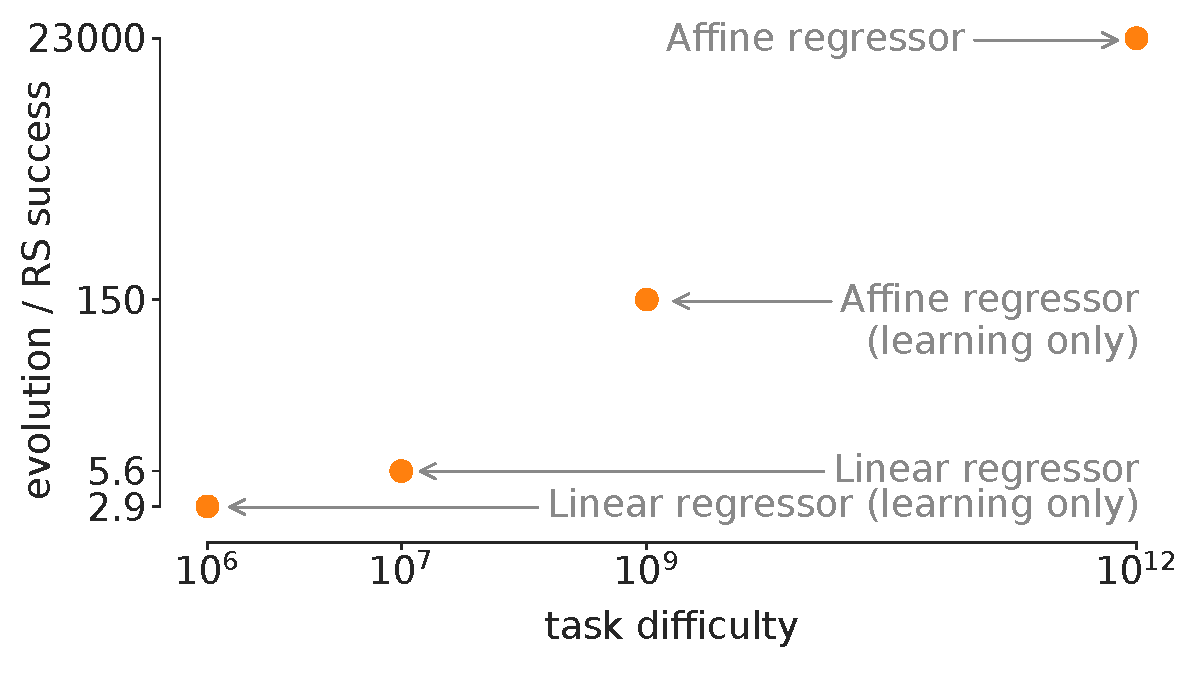
\includegraphics[width=\columnwidth]{relative_difficulty.pdf}}
        \caption{Relative success rate of evolution and random search (RS). Each point represents a different task type and the x-axis measures its difficulty (defined in the main text). As the task type becomes more difficult, evolution vastly outperforms RS, illustrating the complexity of \amlz when compared to more traditional \aml{} spaces.}
        \label{relative_difficulty_fig}
        \vspace{-2pt}
    \end{centering}
\end{figure}

Figure~\ref{relative_difficulty_fig} summarizes the result of this analysis for 4 task types: the discovery of a full-algorithm/only-the-learning for linear/affine regression data. The \amlz search space is generic but this comes at a cost: even for easy problems, good algorithms are sparse. As the problem becomes more difficult, the solutions become vastly more sparse and evolution greatly outperforms RS.

As soon as we advance to nonlinear data, the gap widens and we can no longer find solutions with RS. To make sure a good solution exists, we generate regression tasks using \emph{teacher} neural networks and then verify that evolution can rediscover the teacher's code.

\experimentdetails{tasks as above but the labeling function is now a teacher network:
$L(x_i)\!=\!u\!\cdot\!\textrm{ReLU}(M\!x_i)$, where
$M$ is a random $8\times8$ matrix, $u$ is a random vector. Number of training examples up to $100\textrm{\normalfont{k}}$. Single expt. Same search space restrictions as above, but now allowing ops used in 2-layer fully connected neural nets. After searching, we select the algorithm with the smallest RMS loss. Full configs.\ in Suppl.\ Section~\ref{detailed_experiment_setups_sec}. Note that the restrictions above apply *only* to this section (\ref{difficulty_sec}).}

When the search method uses only 1 task in $\mathcal{T}_{search}$ (\ie $D\!=\!\!1$), the algorithm evolves the exact prediction function used by the teacher and hard-codes its weights. The results become more surprising as we increase the number of tasks in $\mathcal{T}_{search}$ (\eg to $D\!=\!\!100$), as now the algorithm must find different weights for each task. In this case, evolution not only discovers the forward pass, but also ``invents'' back-propagation code to learn the weights (Figure~\ref{nn_fig}). Despite its difficulty, we conclude that searching the \amlz space seems feasible and we should use evolutionary search instead of RS for more complex tasks.

% Source: https://colab.corp.google.com/drive/11juy4K6-5fykzNQG4Xd22q02WmDZxtY7#scrollTo=-0UrxNJIlHQu
% Edited: https://docs.google.com/document/d/1NCcS8jPUgVpV9LW4gwHNoUid6BroYCRAXfxeZFKchAw/edit
\begin{figure}[h]
    \begin{code}{0.48\textwidth}{2.75in}{codebackground}
    \codeline{\codecomment{sX/vX/mX = scalar/vector/matrix at address X.}}
    \codeline{\codecomment{``gaussian'' produces Gaussian IID random numbers.}}
    \codeskip
    \codeline{\codedef{def} Setup():}
      \codeline{\codetab \codecomment{Initialize variables.}}
      \codeline{\codetab m1 = gaussian(-1e-10, 9e-09) \codecomment{1st layer weights}}
      \codeline{\codetab s3 = 4.1 \codecomment{Set learning rate}}
      \codeline{\codetab v4 = gaussian(-0.033, 0.01) \codecomment{2nd layer weights}}    \codeskip
    \codeline{\codedef{def} Predict(): \codecomment{v0=features}}
      \codeline{\codetab v6 = dot(m1, v0) \codecomment{Apply 1st layer weights}}
      \codeline{\codetab v7 = maximum(0, v6) \codecomment{Apply ReLU}}
      \codeline{\codetab s1 = dot(v7, v4) \codecomment{Compute prediction}}
    \codeskip
    \codeline{\codedef{def} Learn(): \codecomment{s0=label}}
      \codeline{\codetab v3 = heaviside(v6, 1.0) \codecomment{ReLU gradient}}
      \codeline{\codetab s1 = s0 - s1 \codecomment{Compute error}}
      \codeline{\codetab s2 = s1 * s3 \codecomment{Scale by learning rate}}
      \codeline{\codetab v2 = s2 * v3 \codecomment{Approx.\ 2nd layer weight delta}}
      \codeline{\codetab v3 = v2 * v4 \codecomment{Gradient w.r.t.\ activations}}
      \codeline{\codetab m0 = outer(v3, v0) \codecomment{1st layer weight delta}} 
      \codeline{\codetab m1 = m1 + m0 \codecomment{Update 1st layer weights}}
      \codeline{\codetab v4 = v2 + v4 \codecomment{Update 2nd layer weights}}
    \end{code}
\caption{Rediscovered neural network algorithm. It implements backpropagation by gradient descent. Comments added manually.}
\label{nn_fig}
\end{figure}

%%%%%%%%%%%%%%%%%%%%%%%%%%%%%%%%%%%%%%%%%%%%%%%%%%%%%%%%%%%%%%%%%%%%%%%%%%%%%%%%%%%%%%%%%%%%%%%%%%
\subsection{Searching with Minimal Human Input}
%%%%%%%%%%%%%%%%%%%%%%%%%%%%%%%%%%%%%%%%%%%%%%%%%%%%%%%%%%%%%%%%%%%%%%%%%%%%%%%%%%%%%%%%%%%%%%%%%%
\label{main_result_sec}

Teacher datasets and carefully chosen ops bias the results in favor of known algorithms, so in this section we replace them with more generic options. We now search among a long list of ops selected based on the simplicity criterion described in Section~\ref{methods_search_space_sec}. The increase in ops makes the search more difficult but allows the discovery of solutions other than neural networks. For more realistic datasets, we use binary classification tasks extracted from CIFAR-10 and MNIST.

\begin{figure*}[!htp]
%%%%%%%%%%%%%%%%%%%%%%%%%%%%%%%%%%%
%%%%%%%%% Progress plot. %%%%%%%%%%
%%%%%%%%%%%%%%%%%%%%%%%%%%%%%%%%%%%
% Experiment Script: https://cs.corp.google.com/piper///depot/google3/experimental/users/evol-brain-gpu/evolution/encodings/crogs/recent_command_lines/2019-01-17.davidso.main_result_reproduce_tp.sh?type=cs&q=2019-01-17.davidso.main_result_reproduce_tp.sh+&g=0&l=1
% Progress: https://colab.corp.google.com/drive/133qUglIq7uW2S3BLblHm6Ewh74bKWr8V#scrollTo=2e0akAYeJiXc
\sbox0{
    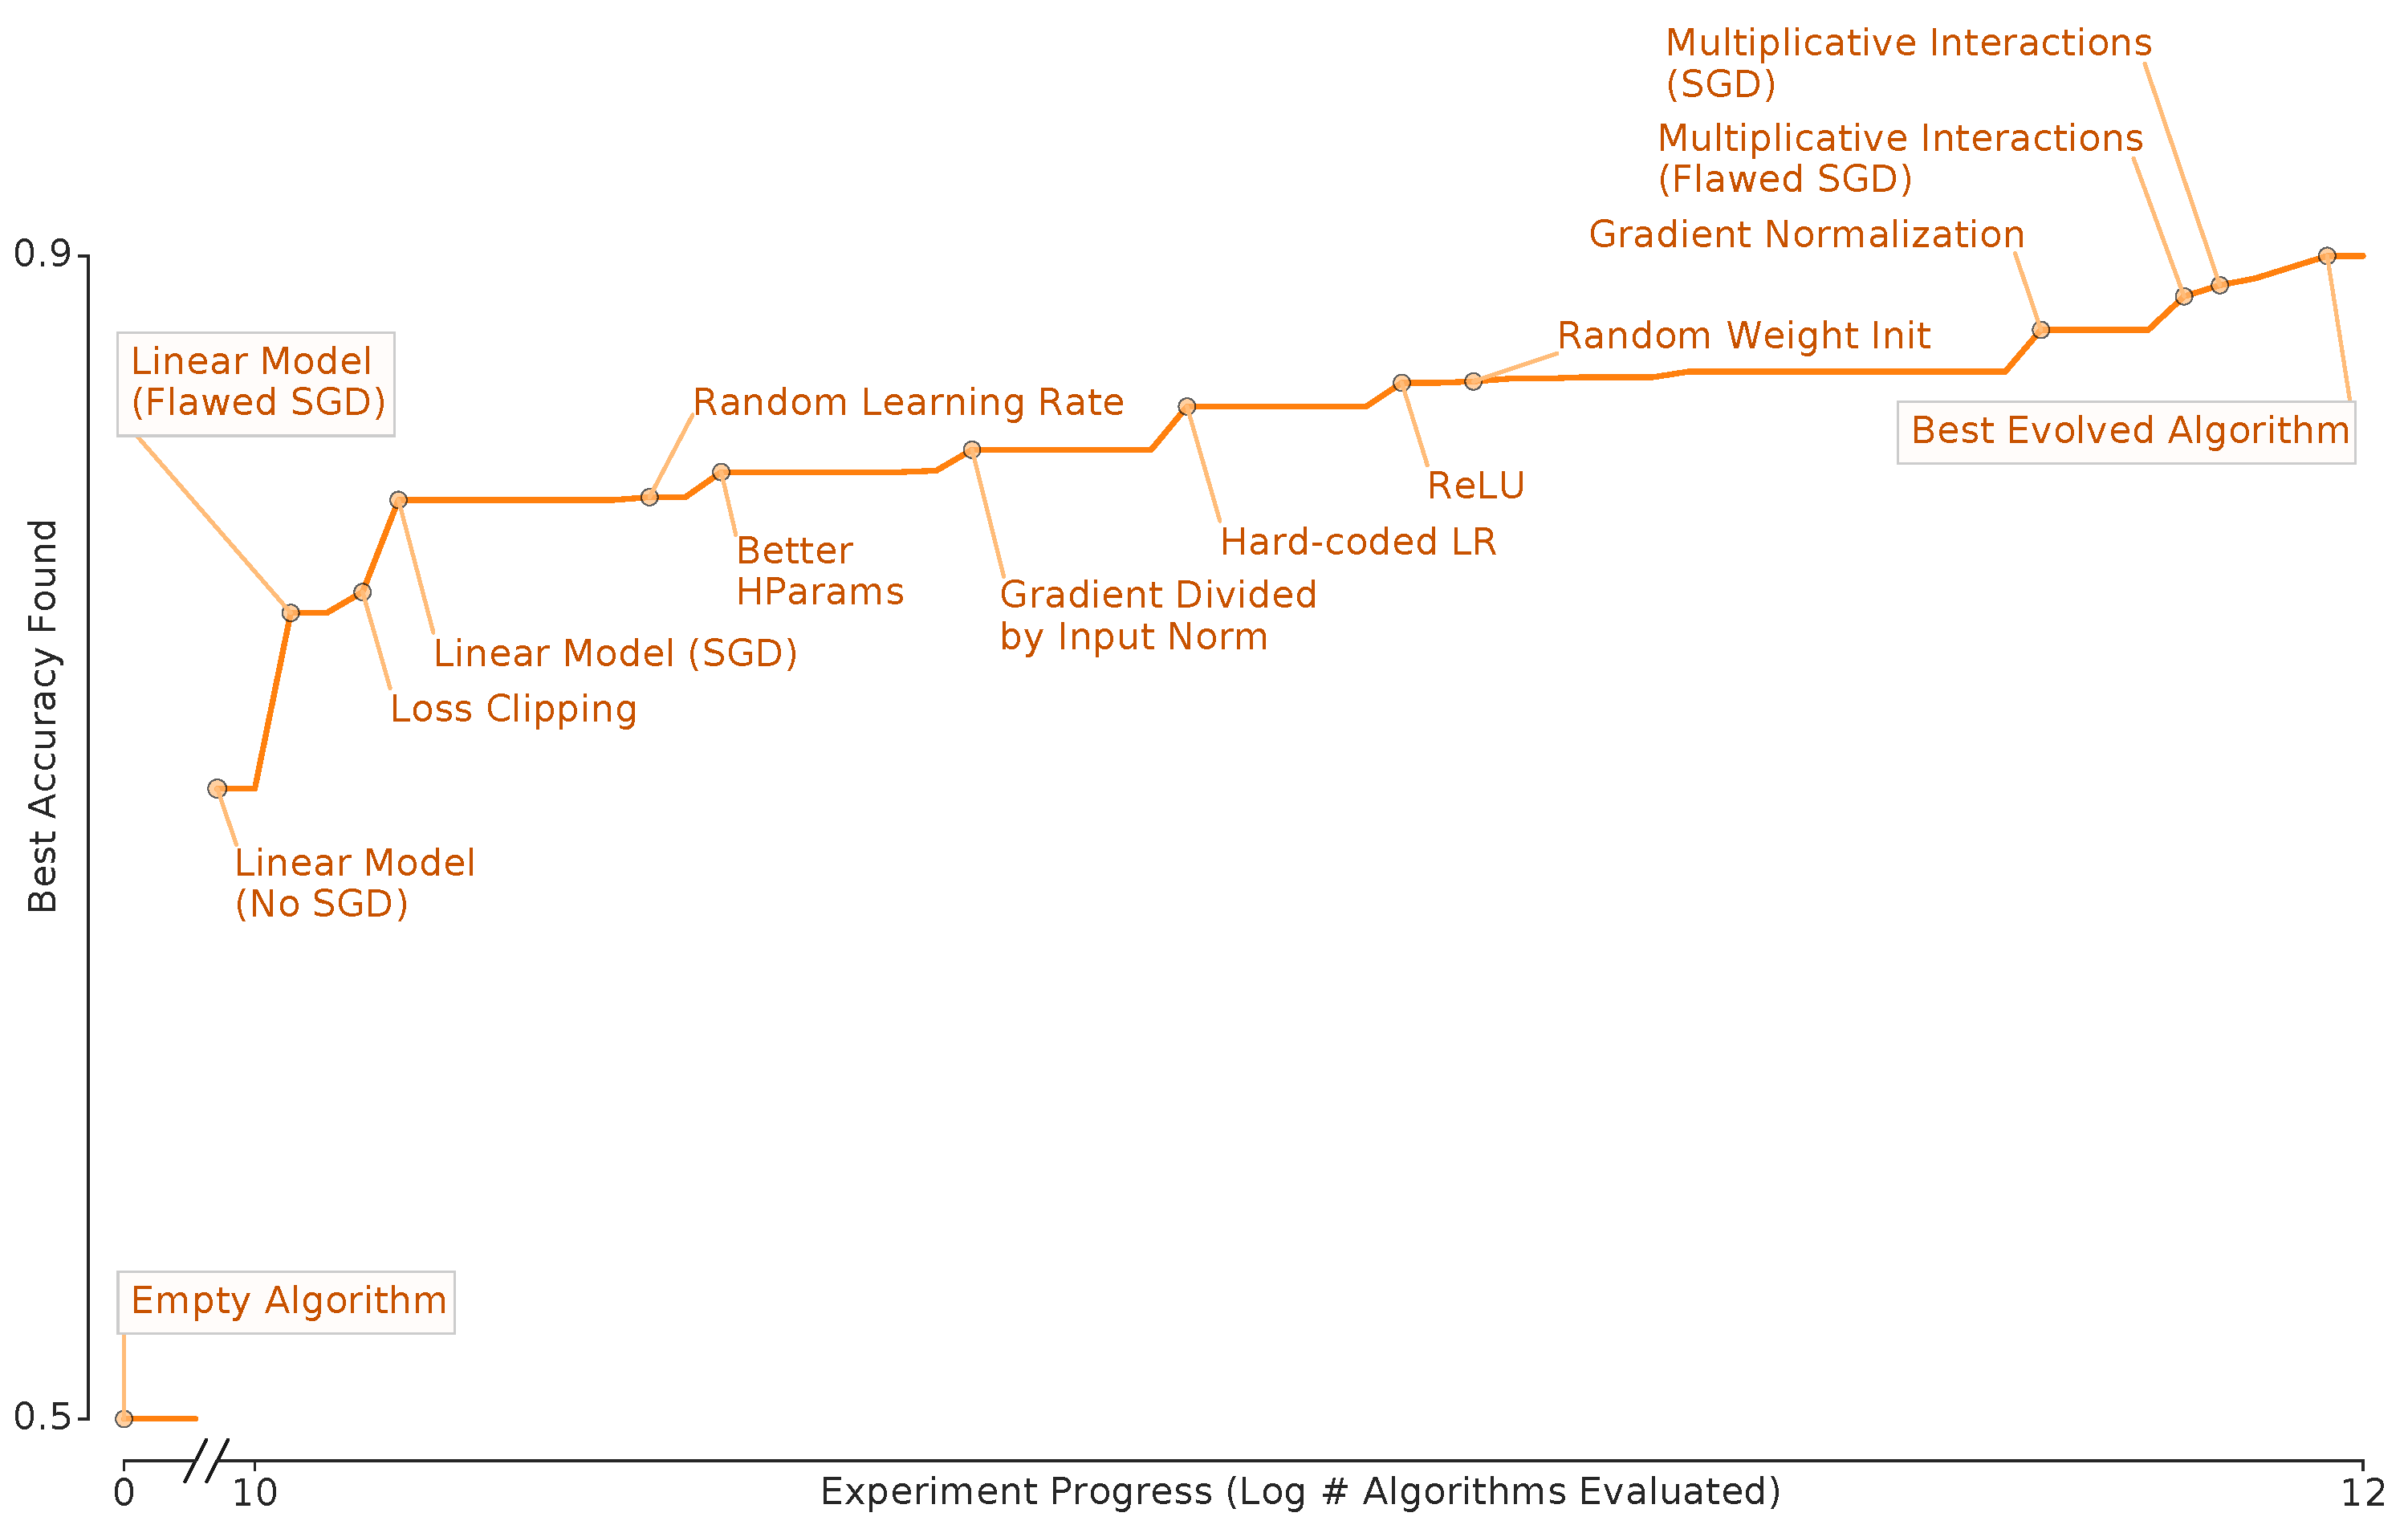
\includegraphics[width=\textwidth, trim=5 0 15 0, clip]{experiment_progress.pdf}%
}
%%%%%%%%%%%%%%%%%%%%%%%%%%%%%%%%%%%%%%%%%%
%%%%%%%%% Empty algorithm code. %%%%%%%%%%
%%%%%%%%%%%%%%%%%%%%%%%%%%%%%%%%%%%%%%%%%%
\sbox1{
    \begin{minipage}{1.2in}
    \begin{code}{\textwidth}{0.88in}{codebackgroundprogress}
    \codeline{\codedef{def} Setup():}
    \codeskip
    \codeline{\codedef{def} Predict():}
    \codeskip
    \codeline{\codedef{def} Learn():}
    \end{code}
    \end{minipage}%
}
%%%%%%%%%%%%%%%%%%%%%%%%%%%%%%%%%%%%%%%%%%%%%%%%%
%%%%%%%%% Intermediate algorithm code. %%%%%%%%%%
%%%%%%%%%%%%%%%%%%%%%%%%%%%%%%%%%%%%%%%%%%%%%%%%%
% Source: https://docs.google.com/document/d/1AgSfaNrvWvAq_paw0E62Tbt_uV8OuSxLEnWfxdavgmE/edit?usp=sharing
\sbox2{
\begin{minipage}{4in}
    \begin{code}{\textwidth}{0.9in}{codebackgroundprogress}
    \begin{minipage}{1.95in}
        \codeline{\codedef{def} Setup():}
        \codeline{\codetab \codecomment{Init weights}}
        \codeline{\codetab v1 = gaussian(0.0, 0.01)}  % Weight init.
        \codeline{\codetab s2 = -1.3}
        \codeskip
        \codeline{\codedef{def} Predict():\ \codecomment{v0=features}}
        \codeline{\codetab s1 = dot(v0, v1) \codecomment{Prediction}}
        \codeskip
    \end{minipage}%
    \begin{minipage}{2in}
        \codeline{\codedef{def} Learn():\ \codecomment{s0=label}}
        \codeline{\codetab s3 = s1 / s2 \codecomment{Scale predict.}}  %Scale down prediction
        \codeline{\codetab s1 = s0 + s3 \codecomment{Compute error}}
        \codeline{\codetab v2 = s1 * v0 \codecomment{Gradient}}
        \codeline{\codetab v1 = v1 + v2 \codecomment{Update weights}}
        \codeline{\ }
    \end{minipage}%
    \end{code}
    \end{minipage}%
}
%%%%%%%%%%%%%%%%%%%%%%%%%%%%%%%%%%%%%%%%%
%%%%%%%%% Best algorithm code. %%%%%%%%%%
%%%%%%%%%%%%%%%%%%%%%%%%%%%%%%%%%%%%%%%%%
% Best algorithm (after ablation studies): https://colab.corp.google.com/drive/14czm6QPIiSVeRIyrgU8KRWM2_sSPay-w#scrollTo=cj_LQVOri6vO&line=9&uniqifier=1
% Best algorithm (raw and after automatic simplification): https://colab.corp.google.com/drive/14czm6QPIiSVeRIyrgU8KRWM2_sSPay-w#scrollTo=q8gO04_NhqDN&line=7&uniqifier=1
\sbox3{
    \begin{minipage}{2.24in}  % Was 2.1in.
    \begin{code}{\textwidth}{2.74in}{codebackgroundprogress}
    \codeline{\codedef{def} Setup():}
    \codeline{\codetab s4 = 1.8e-3 \codecomment{Learning rate}}
    \codeskip
    \codeline{\codedef{def} Predict():\ \codecomment{v0=features}}
        \codeline{\codetab v2 = v0 + v1 \codecomment{Add noise}}
        \codeline{\codetab v3 = v0 - v1 \codecomment{Subtract noise}}
        \codeline{\codetab v4 = dot(m0, v2) \codecomment{Linear}}
        \codeline{\codetab s1 = dot(v3, v4) \codecomment{Mult.interac.}}
        \codeline{\codetab m0 = s2 * m2 \codecomment{Copy weights}}
    \codeskip
    \codeline{\codedef{def} Learn():\ \codecomment{s0=label}}
        \codeline{\codetab s3 = s0 - s1 \codecomment{Compute error}}
        \codeline{\codetab m0 = outer(v3, v0) \codecomment{Approx grad}}
        \codeline{\codetab s2 = norm(m0) \codecomment{Approx grad norm}}
        \codeline{\codetab s5 = s3 / s2 \codecomment{Normalized error}}
        \codeline{\codetab v5 = s5 * v3}
        \codeline{\codetab m0 = outer(v5, v2) \codecomment{Grad}}  % Normalzied grad
        \codeline{\codetab m1 = m1 + m0 \codecomment{Update weights}}
        \codeline{\codetab m2 = m2 + m1 \codecomment{Accumulate wghts.}}
        \codeline{\codetab m0 = s4 * m1}
        \codeline{\codetab \codecomment{Generate noise}}
        \codeline{\codetab v1 = uniform(2.4e-3, 0.67)}
    \end{code}
    \end{minipage}%
}
%%%%%%%%%%%%%%%%%%%%%%%%%%%%%%%%%%%%%%%%%%%%
%%%%%%%%% Best algorithm diagram. %%%%%%%%%%
%%%%%%%%%%%%%%%%%%%%%%%%%%%%%%%%%%%%%%%%%%%%
% Source: https://docs.google.com/presentation/d/1Cd2D1J7Is0saaUoRNsy78ydXCf_qQmWqZ-f7_JqNEeY/edit#slide=id.g7c8ea9320d_0_29
\def\diagramextrawidth{35pt}
\sbox4{
    \begin{minipage}[c]{2in+\diagramextrawidth}
    \centering
    \begin{tcolorbox}[
        width=2in+\diagramextrawidth,height=2in,
        valign=center,left=0pt,right=0pt,top=0pt,bottom=0pt,
        colback=codebackgroundprogress,colframe=codeframe,boxrule=0.5pt,arc=0pt]
    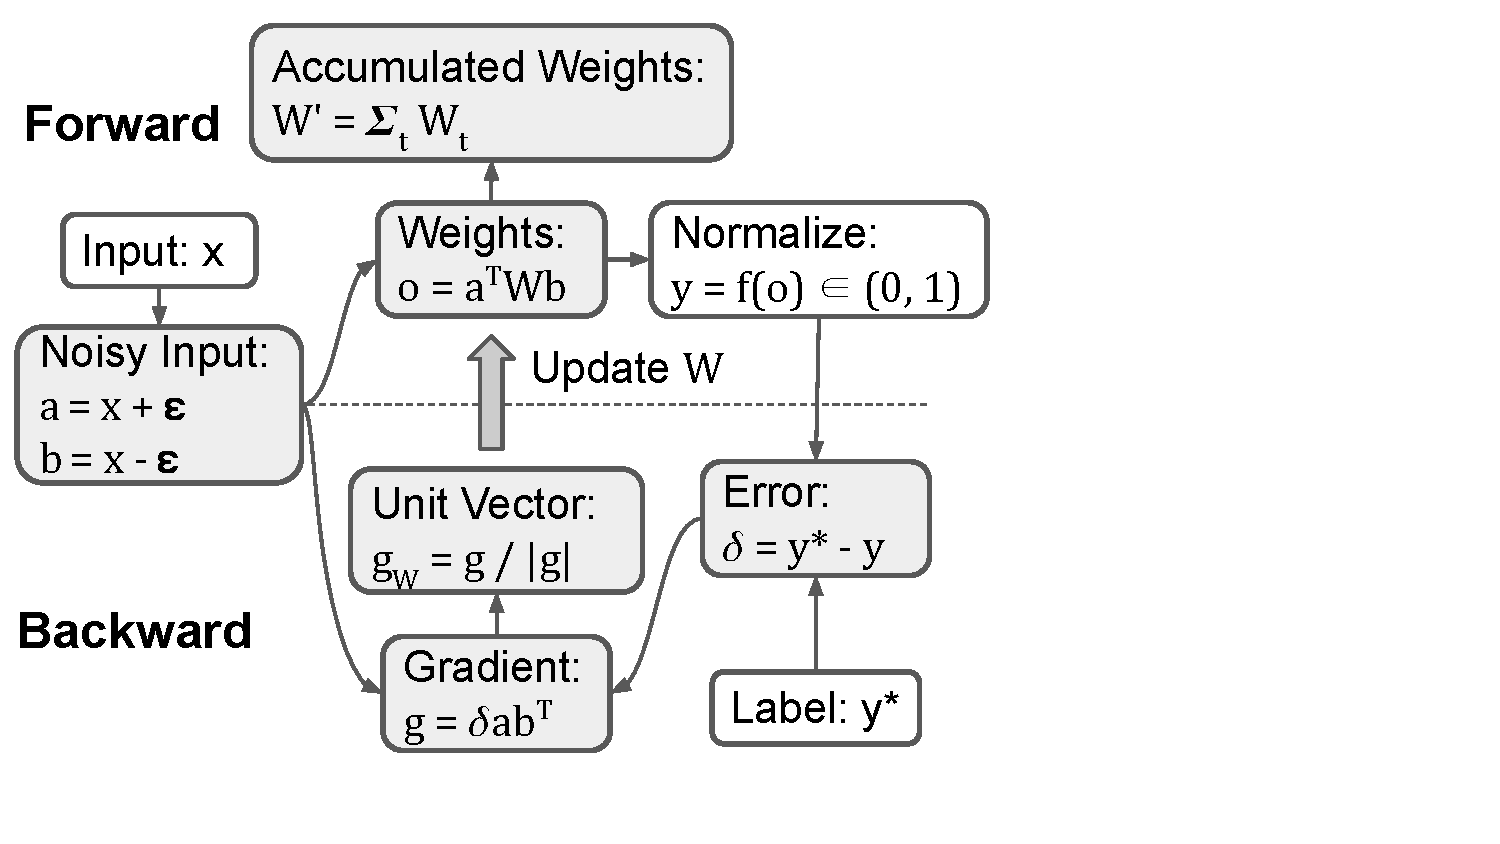
\includegraphics[width=1.9in + \diagramextrawidth, trim=7 40 223 5, clip]{best_algorithm.pdf}
    \end{tcolorbox}
    \end{minipage}
}
%%%%%%%%%%%%%%%%%%%%%%%%%%%%%%%%%%%%%%%%%%%%%%%%%%%%%%%%%%%%%%%
%%%%%%%%% Separator cover for empty algorithm label. %%%%%%%%%%
%%%%%%%%%%%%%%%%%%%%%%%%%%%%%%%%%%%%%%%%%%%%%%%%%%%%%%%%%%%%%%%
\sbox5{
    \begin{tcolorbox}[
        width=68.55pt,height=3pt,
        valign=center,left=0pt,right=0pt,top=0pt,bottom=0pt,
        colback=codebackgroundprogress,colframe=codebackgroundprogress,boxrule=0.5pt,arc=0pt]
    \end{tcolorbox}
}
%%%%%%%%%%%%%%%%%%%%%%%%%%%%%%%%%%%%%%%%%%%%%%%%%%%%%%%%%%%%%%%%
%%%%%%%%% Separator cover for linear algorithm label. %%%%%%%%%%
%%%%%%%%%%%%%%%%%%%%%%%%%%%%%%%%%%%%%%%%%%%%%%%%%%%%%%%%%%%%%%%%
\sbox6{
    \begin{tcolorbox}[
        width=56.4pt,height=3pt,
        valign=center,left=0pt,right=0pt,top=0pt,bottom=0pt,
        colback=codebackgroundprogress,colframe=codebackgroundprogress,boxrule=0.5pt,arc=0pt]
    \end{tcolorbox}
}
%%%%%%%%%%%%%%%%%%%%%%%%%%%%%%%%%%%%%%%%%%%%%%%%%%%%%%%%%%%%%%%%
%%%%%%%%% Separator cover for best algorithm diagram. %%%%%%%%%%
%%%%%%%%%%%%%%%%%%%%%%%%%%%%%%%%%%%%%%%%%%%%%%%%%%%%%%%%%%%%%%%%
\sbox8{
    \begin{tcolorbox}[
        width=3pt,height=143.4pt,
        valign=center,left=0pt,right=0pt,top=0pt,bottom=0pt,
        colback=codebackgroundprogress,colframe=codebackgroundprogress,boxrule=0.5pt,arc=0pt]
    \end{tcolorbox}
}
%%%%%%%%%%%%%%%%%%%%%%%%%%%%%%%%%%%%%%%%%%%%%%%%%%%%%%%%%%%%%%
%%%%%%%%% Separator cover for best algorithm label. %%%%%%%%%%
%%%%%%%%%%%%%%%%%%%%%%%%%%%%%%%%%%%%%%%%%%%%%%%%%%%%%%%%%%%%%%
\sbox9{
    \begin{tcolorbox}[
%%%%%%%%%%%%%%%%%%%%%%%%%%%%%%%%%%%%%%%%%%%%%%%%%%%%%%%%%%%%%%%%%%%%%%%%%%%%%%%%%%%%%%%%%%%%%%%%%%%%%%%%%%%
%%%%%%%%%%%%%%%%%%%%%%%%%%%%%%%%%%%%%%%%%%%%%%%%%%%%%%%%%%%%%%%%%%%%%%%%%%%%%%%%%%%%%%%%%%%%%%%%%%%%%%%%%%%
%%%%%%%%%%%%%%%%%%%%%%%%%%%%%%%%%%%%%%%%%%%%%%%%%%%%%%%%%%%%%%%%%%%%%%%%%%%%%%%%%%%%%%%%%%%%%%%%%%%%%%%%%%%
        width=93.4pt,height=3pt,
        valign=center,left=0pt,right=0pt,top=0pt,bottom=0pt,
        colback=codebackgroundprogress,colframe=codebackgroundprogress,boxrule=0.5pt,arc=0pt]
%%%%%%%%%%%%%%%%%%%%%%%%%%%%%%%%%%%%%%%%%%%%%%%%%%%%%%%%%%%%%%%%%%%%%%%%%%%%%%%%%%%%%%%%%%%%%%%%%%%%%%%%%%%
%%%%%%%%%%%%%%%%%%%%%%%%%%%%%%%%%%%%%%%%%%%%%%%%%%%%%%%%%%%%%%%%%%%%%%%%%%%%%%%%%%%%%%%%%%%%%%%%%%%%%%%%%%%
%%%%%%%%%%%%%%%%%%%%%%%%%%%%%%%%%%%%%%%%%%%%%%%%%%%%%%%%%%%%%%%%%%%%%%%%%%%%%%%%%%%%%%%%%%%%%%%%%%%%%%%%%%%
    \end{tcolorbox}
}
%%%%%%%%%%%%%%%%%%%%%%%%%%%%%%%%%%%%
%%%%%%%%% Complete figure.%%%%%%%%%%
%%%%%%%%%%%%%%%%%%%%%%%%%%%%%%%%%%%%
%
% History graph: https://colab.corp.google.com/drive/133qUglIq7uW2S3BLblHm6Ewh74bKWr8V#scrollTo=jvg0k2P8VcH4
\createlength{\diagramshift}{92.9pt - \diagramextrawidth}  % Was 102.9pt.
\hspace*{-6pt}
\usebox0%  % Background
\raisebox{81.8pt}{\hspace*{-468.1pt}\usebox1}\hspace*{0.2in}%  % Empty algorithm code  % 266pt
\raisebox{51pt}{\hspace*{-103.1pt}\usebox5}%  % Separator cover for empty algorithm label
\raisebox{274pt}{\hspace*{-74.175pt}\usebox2}%  % Linear algorithm code
\raisebox{243pt}{\hspace*{-291.05pt}\usebox6}%  % Separator cover for linear algorithm label
\raisebox{92.3pt}{\hspace*{\diagramshift}\usebox4}%  % Final algorithm diagram
\raisebox{119pt}{\hspace*{-6pt}\usebox3}%  % Final algorithm code
\raisebox{23pt}{\hspace*{-166pt}\usebox8}%  % Separator cover for final algorithm diagram
\raisebox{218pt}{\hspace*{61.8pt}\usebox9}%  % Separator cover for final algorithm label
\caption{Progress of one evolution experiment on projected binary CIFAR-10. Callouts indicate some beneficial discoveries. We also print the code for the initial, an intermediate, and the final algorithm. The last is explained in the flow diagram. It outperforms a simple fully connected neural network on held-out test data and transfers to features 10x its size. Code notation is the same as in Figure~\ref{nn_fig}. The x-axis gap is due to infrequent recording due to disk throughput limitations.}
\label{experiment_progress_fig}
\end{figure*}

\experimentdetails{We extract tasks from the CIFAR-10 and MNIST training sets; each of the datasets are searched on by half of the processes. For both datasets, the 45 pairs of the 10 classes yield tasks with $8000$ train\,/\,$2000$ valid examples. $36$ pairs are randomly selected to constitute $\mathcal{T}_{search}$, \ie search tasks; $9$ pairs are held out for $\mathcal{T}_{select}$, \i.e tasks for model selection. The CIFAR-10 test set is reserved for final evaluation to report results. Features are projected to $8 \leq F \leq 256$ dim. Each evaluation is on $1 \leq D \leq 10$ tasks. $W\!\!=\!\!10\textrm{k}$. From now on, we use the full setup described in Section~\ref{methods_search_sec}. In particular, we allow variable component function length. Number of possible ops: $7$/\,$58$/\,$58$ for \setup/\,\predict/\,\learn, resp. Full config.\ in Suppl.\ Section~\ref{detailed_experiment_setups_sec}.}

Figure~\ref{experiment_progress_fig} shows the progress of an experiment. It starts with a population of empty programs and automatically invents improvements, several of which are highlighted in the plot. These intermediate discoveries are stepping stones available to evolution and they explain why evolution outperforms RS in this space. 
Each experiment produces a candidate algorithm using $\mathcal{T}_{search}$. 
We then evaluate these algorithms on unseen pairs of classes ($\mathcal{T}_{select}$) and compare the results to a hand-designed reference, a 2-layer fully connected neural network trained by gradient descent. The candidate algorithms perform better in 13 out of 20 experiments. To make sure the improvement is not specific to the small proxy tasks, we select the best algorithm for a final evaluation on binary classification with the original CIFAR-10 data.

%source of eval results:
%https://docs.google.com/spreadsheets/d/1IRyF3_UvkiZo6LFFx7Sh70IBOBU_PHKgwkMJGWeDPLA/edit#gid=0
%https://colab.corp.google.com/drive/14x2BkFxA2jvF-VA8GWxxnB3-ncLGwwih#scrollTo=EU7nCt5NaOSu&line=67&uniqifier=1
Since we are evaluating on tasks with different dimensionality in the final evaluation, we treat all the constants in the best evolved algorithm as hyperparameters and tune them jointly through RS using the validation set. For comparison, we tune two hand-designed baselines, one linear and one nonlinear, using the same total compute that went into discovering and tuning the evolved algorithm. We finally evaluate them all on unseen CIFAR-10 test data. Evaluating with 5 different random seeds, the best evolved algorithm's accuracy ($84.06\pm0.10\%$) significantly outperforms the linear baseline (logistic regression, $77.65\pm0.22\%$) and the nonlinear baseline (2-layer fully connected neural network, $82.22\pm0.17\%$). This gain also generalizes to binary classification tasks extracted from other datasets: SVHN~\cite{netzer2011reading} ($88.12\%$ for the best evolved algorithm \vs $59.58\%$ for the linear baseline \vs $85.14\%$ for the nonlinear baseline), downsampled ImageNet~\cite{chrabaszcz2017downsampled} ($80.78\%$ \vs $76.44\%$ \vs $78.44\%$), Fashion MNIST~\cite{xiao2017fashion} ($98.60\%$ \vs $97.90\%$ \vs $98.21\%$). This algorithm is limited by our simple search space, which cannot currently represent some techniques that are crucial in state-of-the-art models, like batch normalization or convolution. Nevertheless, the algorithm shows interesting characteristics, which we describe below.

\begin{figure*}[!hb]
%%%%%%%%%%%%%%%%%%%%%%%%%%%%%%%%%%%%%%%%%%%%%
%%%%%%%%% Noisy ReLU code snippet. %%%%%%%%%%
%%%%%%%%%%%%%%%%%%%%%%%%%%%%%%%%%%%%%%%%%%%%%
\createlength{\firstrowheight}{1.73in}  % Was 1.73in
\createlength{\secondrowheight}{1in}  % Was 1in.
\createlength{\firstcolwidth}{2.578in}
\createlength{\secondcolwidth}{1.597in}
\createlength{\thirdcolwidth}{2.316in}
\createlength{\subcaptionspacing}{-10pt}
\def\rowsep{\medskip}
\def\adaptcodesubref{top}
\def\adaptdiagramsubref{bottom}
\sbox0{\begin{subfigure}[@{}c]{\firstcolwidth}
    % source: https://colab.corp.google.com/drive/14czm6QPIiSVeRIyrgU8KRWM2_sSPay-w#scrollTo=a2P4tT_9SyPw&line=7&uniqifier=1
    % comparison to control experiments: https://colab.corp.google.com/drive/14czm6QPIiSVeRIyrgU8KRWM2_sSPay-w#scrollTo=RpYOXk7zdlCy&line=8&uniqifier=1
    % experiment script: https://cs.corp.google.com/piper///depot/google3/experimental/users/evol-brain-gpu/evolution/encodings/crogs/recent_command_lines/2019-12-26.crazydonkey.gf_small_data.sh
    \begin{code}{\firstcolwidth}{\firstrowheight}{codebackground}
    \codeline{\codedef{def} Predict():}
        \codeline{\codetab ... \codecomment{Omitted/irrelevant code}}
        \codeline{\codetab \codecomment{v0=features; m1=weight matrix}}
        \codeline{\codetab v6 = dot(m1, v0) \codecomment{Apply weights}}
        \codeline{\codetab \codecomment{Random vector, \textmu=-0.5 and \textsigma=0.41}}
        \codeline{\codetab v8 = gaussian(-0.5, 0.41)}
        \codeline{\codetab v6 = v6 + v8 \codecomment{Add it to activations}}
        \codeline{\codetab v7 = maximum(v9, v6) \codecomment{ReLU, v9$\approx$0}}
        \codeline{\codetab ...}
        \codeline{\ }
        \codeline{\ }
        \codeline{\ }
        \codeline{\ }
    \end{code}
\end{subfigure}}
%%%%%%%%%%%%%%%%%%%%%%%%%%%%%%%%%%%%%%%%%%%
%%%%%%%%% LR decay code snippet. %%%%%%%%%%
%%%%%%%%%%%%%%%%%%%%%%%%%%%%%%%%%%%%%%%%%%%
\sbox1{\begin{subfigure}[@{}c]{\secondcolwidth}
    % source: https://colab.corp.google.com/drive/14czm6QPIiSVeRIyrgU8KRWM2_sSPay-w#scrollTo=6QlhTA_kShQh&line=5&uniqifier=1
    % comparison to control experiments: https://colab.corp.google.com/drive/14czm6QPIiSVeRIyrgU8KRWM2_sSPay-w#scrollTo=Xz1GRIlzbDy2&line=7&uniqifier=1
    % experiment script: https://cs.corp.google.com/piper///depot/google3/experimental/users/evol-brain-gpu/evolution/encodings/crogs/recent_command_lines/2020-01-24.crazydonkey.gf_tr800_ep10_all.sh
    \begin{code}{\secondcolwidth}{\firstrowheight}{codebackground}
    \codeline{\codedef{def} Setup():}
        \codeline{\codetab \codecomment{LR = learning rate}}
        \codeline{\codetab s2 = 0.37 \codecomment{Init.\ LR}}
        \codeline{\codetab ...}
    \codeskip
    \codeline{\codedef{def} Learn():}
        \codeline{\codetab \codecomment{Decay LR}}
        \codeline{\codetab s2 = arctan(s2)}
        \codeline{\codetab ...}
        \codeline{\ }
        \codeline{\ }
        \codeline{\ }
        \codeline{\ }
        \codeline{\ }
    \end{code}
\end{subfigure}}
%%%%%%%%%%%%%%%%%%%%%%%%%%%%%%%%%%%%%%%%%%%%%
%%%%%%%%% LR trick code snippet.   %%%%%%%%%%
%%%%%%%%%%%%%%%%%%%%%%%%%%%%%%%%%%%%%%%%%%%%%
\sbox2{\begin{subfigure}[@{}c]{\thirdcolwidth}
    % source: https://colab.corp.google.com/drive/14czm6QPIiSVeRIyrgU8KRWM2_sSPay-w#scrollTo=rhGS2t4BXnSC&line=7&uniqifier=1
    % comparison to control experiments: https://colab.corp.google.com/drive/14czm6QPIiSVeRIyrgU8KRWM2_sSPay-w#scrollTo=utrl6e_ZY2HX&line=30&uniqifier=1
    % experiment script: https://cs.corp.google.com/piper///depot/google3/experimental/users/evol-brain-gpu/evolution/encodings/crogs/recent_command_lines/2020-01-10.crazydonkey.gf_multiclass-d16-standard-1.sh
    \begin{code}{\thirdcolwidth}{\firstrowheight}{codebackground}
    \codeline{\codedef{def} Learn():}
        \codeline{\codetab s3 = mean(m1) \codecomment{m1 is the weights.}}
        \codeline{\codetab s3 = abs(s3)}
        \codeline{\codetab s3 = sin(s3)}
        \codeline{\codetab \codecomment{From here down, s3 is used as}}
        \codeline{\codetab \codecomment{the learning rate.}}
        \codeline{\codetab ...}
        \codeline{\ }
        \codeline{\ }
        \codeline{\ }
        \codeline{\ }
        \codeline{\ }
    \end{code}
\end{subfigure}}
%%%%%%%%%%%%%%%%%%%%%%%%%%%%%%%%%%%%%%%%
%%%%%%%%% Noisy ReLU diagram. %%%%%%%%%%
%%%%%%%%%%%%%%%%%%%%%%%%%%%%%%%%%%%%%%%%
\sbox3{\begin{subfigure}[@{}c]{\firstcolwidth}
    \centering
    \begin{minipage}[c][\secondrowheight][c]{\firstcolwidth}
        \centering
        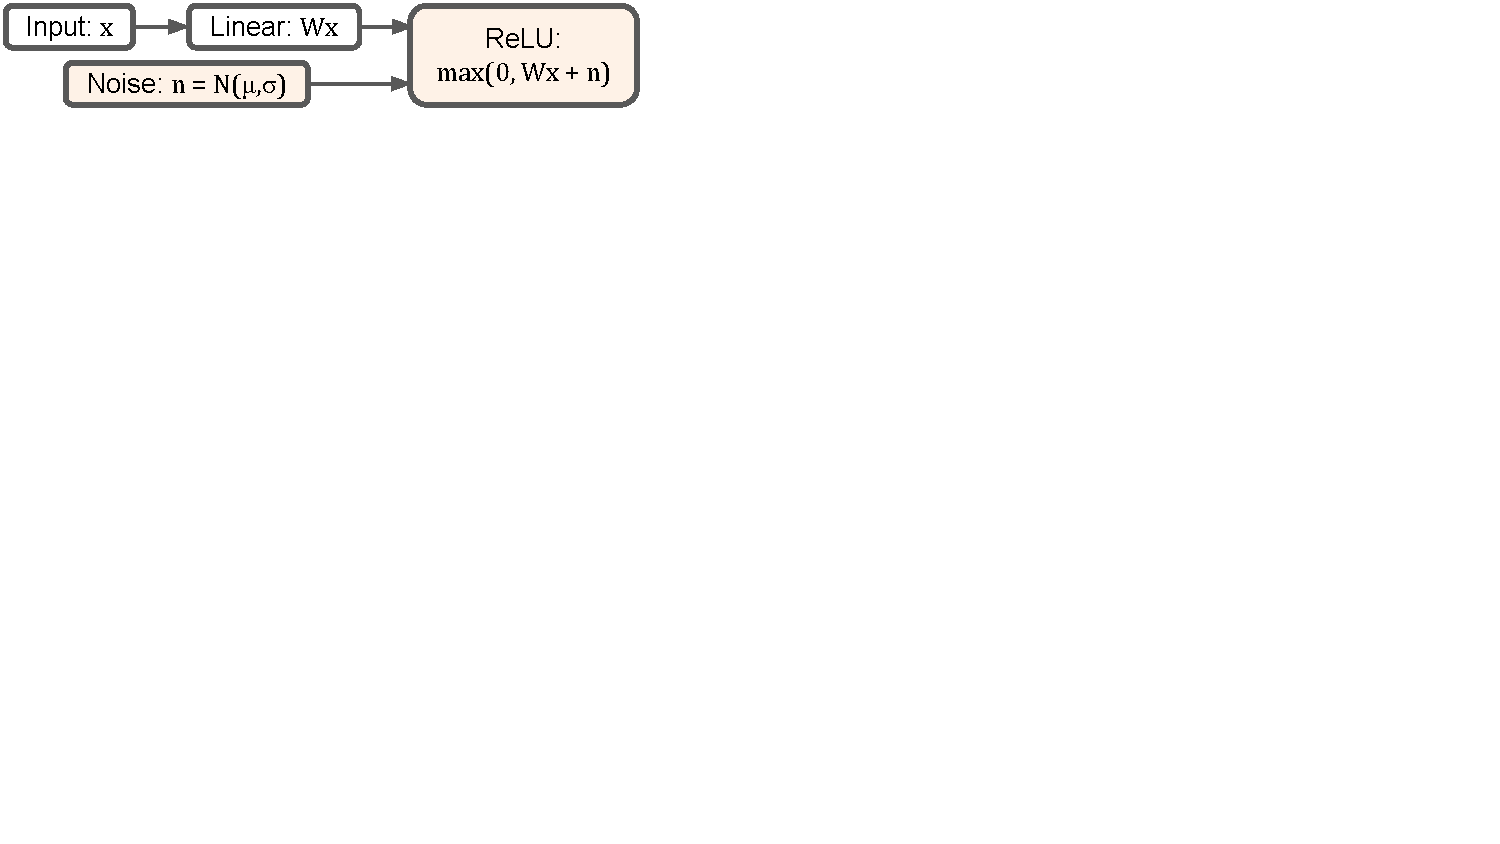
\includegraphics[width=0.97\firstcolwidth, trim=1 352 412 1, clip]{noisy_relu.pdf}
    \end{minipage}
\end{subfigure}}
%%%%%%%%%%%%%%%%%%%%%%%%%%%%%%%%%%%%%%
%%%%%%%%% LR decay diagram. %%%%%%%%%%
%%%%%%%%%%%%%%%%%%%%%%%%%%%%%%%%%%%%%%
% https://colab.corp.google.com/drive/14x2BkFxA2jvF-VA8GWxxnB3-ncLGwwih#scrollTo=UXGaqN6c8UOx&line=44&uniqifier=1
\sbox4{\begin{subfigure}[@{}c]{\secondcolwidth}
    \centering
    \begin{minipage}[c][\secondrowheight][c]{\secondcolwidth}
        \centering
        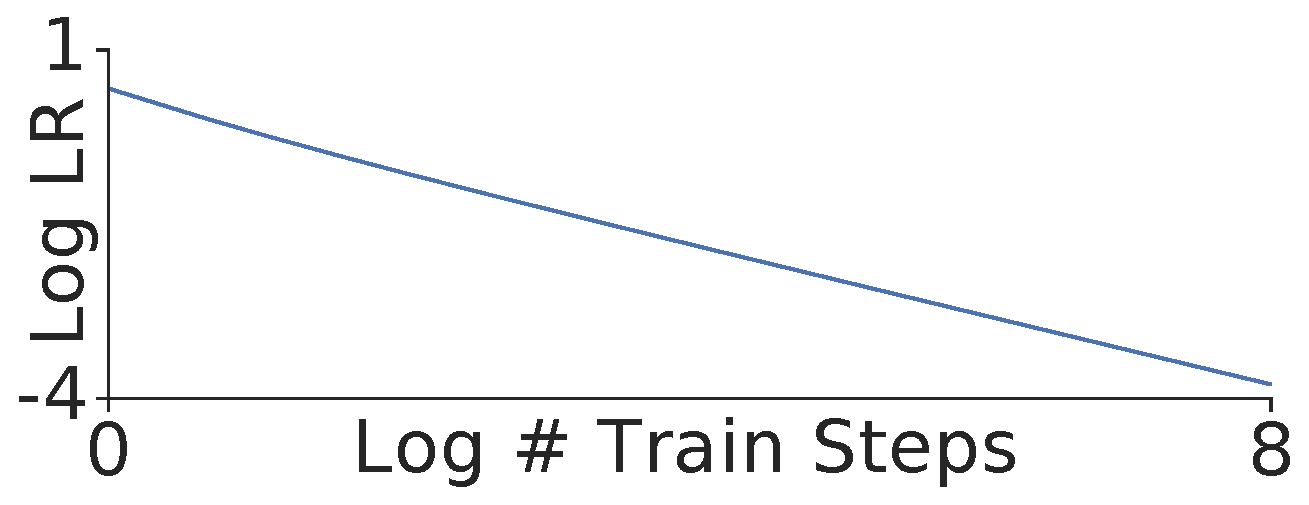
\includegraphics[width=0.95\secondcolwidth, trim=10 5 10 10, clip]{arctan_learning_rate_decay.pdf}
    \end{minipage}
\end{subfigure}}
%%%%%%%%%%%%%%%%%%%%%%%%%%%%%%%%%%%%%%%%
%%%%%%%%% Norm trick diagram. %%%%%%%%%%
%%%%%%%%%%%%%%%%%%%%%%%%%%%%%%%%%%%%%%%%
% Source: https://docs.google.com/presentation/d/1Cd2D1J7Is0saaUoRNsy78ydXCf_qQmWqZ-f7_JqNEeY/edit#slide=id.g6e693cff00_0_0
\sbox5{\begin{subfigure}[@{}c]{\thirdcolwidth}
    \centering
    \begin{minipage}[c][\secondrowheight][c]{\thirdcolwidth}
        \centering
        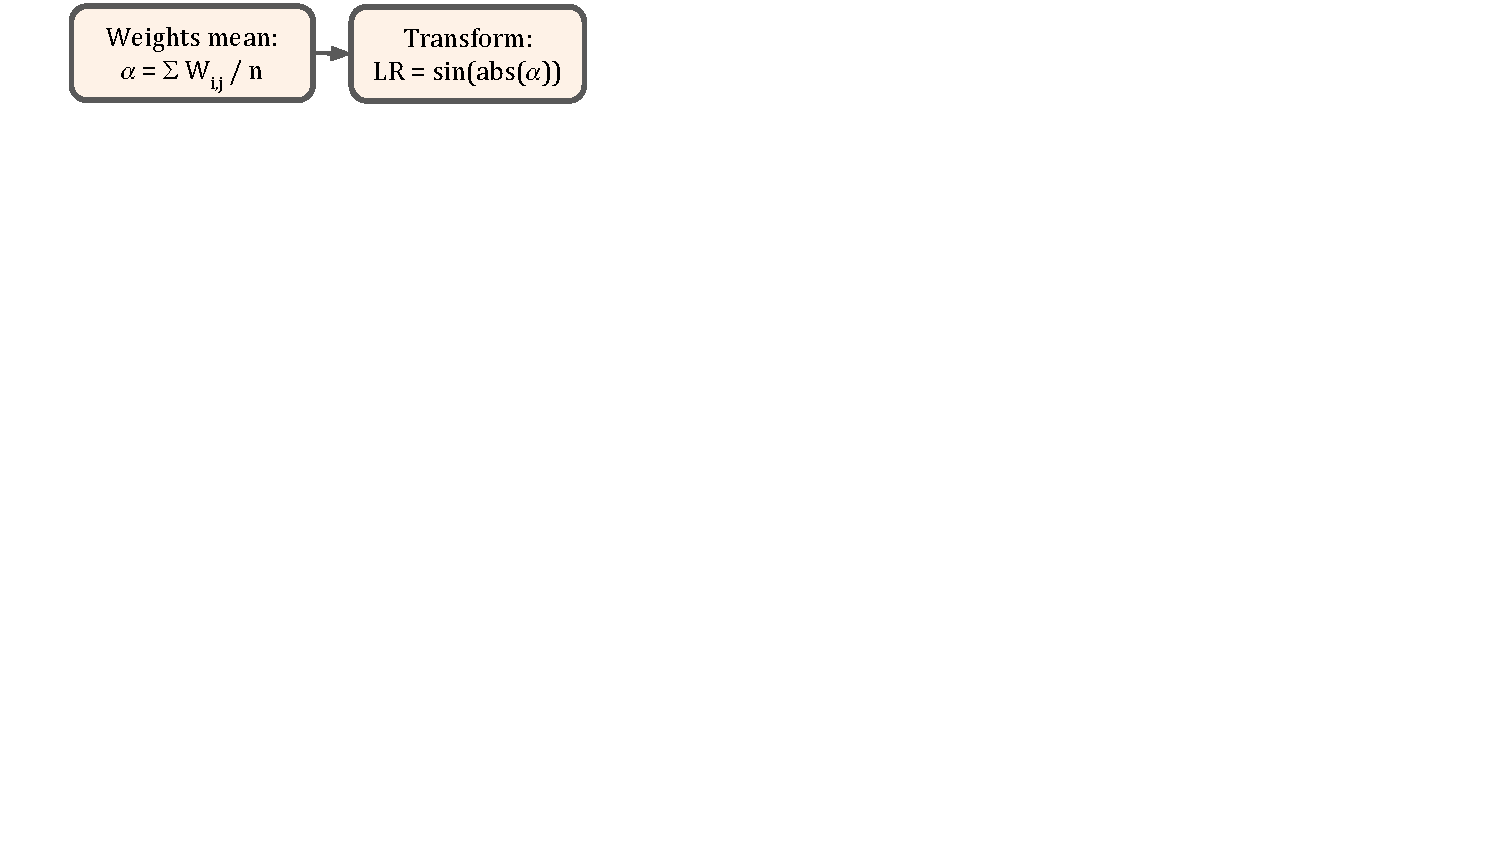
\includegraphics[width=0.97\thirdcolwidth, trim=28 355 437 0, clip]{normalization.pdf}
    \end{minipage}
\end{subfigure}}
\setlength{\tabcolsep}{0pt}
%%%%%%%%%%%%%%%%%%%%%%%%%%%%%%%%%%%%%%%%%%%%%
%%%%%%%%% All about the noisy ReLU.%%%%%%%%%%
%%%%%%%%%%%%%%%%%%%%%%%%%%%%%%%%%%%%%%%%%%%%%
\sbox6{\begin{subfigure}[t]{\firstcolwidth}
    \centering
    \usebox0%  % Noisy ReLU code.
    \raisebox{-44pt}{\hspace*{-186pt}\usebox3}%  % Noisy ReLU diagram.
    \vspace{-14pt}
    \caption{Adaptation to few examples.}
    \label{adapt_noisy_relu_fig}
\end{subfigure}}
%%%%%%%%%%%%%%%%%%%%%%%%%%%%%%%%%%%%%%%%%%%
%%%%%%%%% All about the LR decay.%%%%%%%%%%
%%%%%%%%%%%%%%%%%%%%%%%%%%%%%%%%%%%%%%%%%%%
\sbox7{\begin{subfigure}[t]{\secondcolwidth}
    \centering
    \usebox1%  % LR decay code.
    \raisebox{-40pt}{\hspace*{-115pt}\usebox4}%  % LR decay diagram.
    \vspace{\subcaptionspacing}
    \caption{Adaptation to fast training.}
    \label{adapt_lr_decay_fig}
\end{subfigure}}
%%%%%%%%%%%%%%%%%%%%%%%%%%%%%%%%%%%%%%%%%%%%%
%%%%%%%%% All about the norm trick.%%%%%%%%%%
%%%%%%%%%%%%%%%%%%%%%%%%%%%%%%%%%%%%%%%%%%%%%
\sbox8{\begin{subfigure}[t]{\thirdcolwidth}
    \centering
    \usebox2%  % Norm trick code.
    \raisebox{-40pt}{\hspace*{-168pt}\usebox5}%  % Norm trick diagram.
    \vspace{\subcaptionspacing}
    \caption{Adaptation to multiple classes.}
    \label{adapt_norm_trick_fig}
\end{subfigure}}
%%%%%%%%%%%%%%%%%%%%%%%%%%%%%%%%%%%%
%%%%%%%%% Complete figure.%%%%%%%%%%
%%%%%%%%%%%%%%%%%%%%%%%%%%%%%%%%%%%%
\begin{tabular*}{\linewidth}{@{}@{\extracolsep{\fill}}ccc}
\usebox6 & \usebox7 & \usebox8\\
\end{tabular*}
\caption{Adaptations to different task types. (\subref{adapt_noisy_relu_fig})~When few examples are available, evolution creates a noisy ReLU. (\subref{adapt_lr_decay_fig})~When fast training is needed, we get a learning rate decay schedule implemented as an iterated arctan map (\adaptcodesubref) that is nearly exponential (\adaptdiagramsubref). (\subref{adapt_norm_trick_fig})~With multiple classes, the mean of the weight matrix is transformed and then used as the learning rate. Same notation as in Figure~\ref{nn_fig}; full algorithms in Suppl.\ Section~\ref{full_evolved_algorithms_sec}.}
\label{adapt_fig}
\end{figure*}

As a case study, we delve into the best algorithm, shown in Figure~\ref{experiment_progress_fig}. The code has been cleaned for readability; we removed and rearranged instructions when this caused no difference in performance (raw code in Suppl.\  Section~\ref{full_evolved_algorithms_sec}). The algorithm has the following notable features, whose usefulness we verified through ablations (more details in Suppl.\ Section ~\ref{interpretation_supp_sec}):
(1) Noise is added to the input, which, we suspect, acts as a regularizer: 
\begin{equation*}
\mathbf{a} = \mathbf{x} + \mathbf{u}; \mathbf{b} = \mathbf{x} - \mathbf{u}; \mathbf{u} \sim \mathbf{U}(\alpha, \beta)
\end{equation*}
where $\mathbf{x}$ is the input, $\mathbf{u}$ is a random vector drawn from a uniform distribution. 
(2) Multiplicative interactions \cite{jayakumar2020multiplicative} emerge in a \emph{bilinear} form:
$\mathbf{o} = \mathbf{a}^\intercal \mathbf{W} \mathbf{b}$, 
where $\mathbf{o}$ is the output, and $\mathbf{W}$ is the weight matrix.
(3) The gradient $\mathbf{g}$ \wrt the weight matrix $\mathbf{W}$ is computed correctly and is then normalized to be a unit vector:
\begin{equation*}
    \mathbf{g_w} = \frac{\mathbf{g}}{|\mathbf{g}|}; \mathbf{g} = \mathbf{\delta} \mathbf{a} \mathbf{b}^\intercal; \, \mathbf{\delta} = \mathbf{y^*} -  \mathbf{y}; 
\end{equation*}
where $\mathbf{\delta}$ is the error, $y$ is the predicted probability, and $y^*$ is the label. Normalizing gradients is a common heuristic in non-convex optimization~\cite{hazan2015beyond,levy2016power}.
%, which could help with the vanishing and exploding gradient problem~\cite{yu2017block,pascanu2013difficulty}.
(4) The weight matrix $\mathbf{W'}$ used during inference is the accumulation of all the weight matrices $\{\mathbf{W_t}\}$ after each training step $\mathbf{t}$, \ie: $\mathbf{W'} = \sum_t \mathbf{W_t}$.
This is reminiscent of the \emph{averaged perceptron} \cite{collins2002discriminative} and neural network \emph{weight averaging} during training \cite{polyak1992acceleration,goodfellow2016deep}. Unlike these studies, the evolved algorithm \emph{accumulates} instead of averaging, but this difference has no effect when measuring the accuracy of classification tasks (it does not change the prediction).
As in those techniques, different weights are used at training and validation time. The evolved algorithm achieves this by setting the weights $\mathbf{W}$ equal to $\mathbf{W'}$ at the end of the \predict component function and resetting them to $\mathbf{W_t}$ right after that, at the beginning of the \learn component function. This has no effect during training, when \predict and \learn alternate in execution. However, during validation, \learn is never called and \predict is executed repeatedly, causing $\mathbf{W}$ to remain as $\mathbf{W'}$.

In conclusion, even though the task used during search is simple, the results
%aggregate metrics and case study presented 
show that our framework can discover commonly used algorithms from scratch. 
%discover algorithms that reach the level of human designs, from scratch.

%%%%%%%%%%%%%%%%%%%%%%%%%%%%%%%%%%%%%%%%%%%%%%%%%%%%%%%%%%%%%%%%%%%%%%%%%%%%%%%%%%%%%%%%%%%%%%%%%%
\subsection{Discovering Algorithm Adaptations}
%%%%%%%%%%%%%%%%%%%%%%%%%%%%%%%%%%%%%%%%%%%%%%%%%%%%%%%%%%%%%%%%%%%%%%%%%%%%%%%%%%%%%%%%%%%%%%%%%%
\label{zoo_sec}
% Experiment results: https://docs.google.com/presentation/d/19CbXyw3xtbHtJ_H_clqIpGn3-V-yijWwILwcp5S7Crw/edit?ts=5e2fe683#slide=id.g6dc6f30182_0_37
% Confidence calculations: https://colab.corp.google.com/drive/1I6u4c6pPvLgnRAwfL28QauVZmPwI_57r

In this section, we will show wider applicability by searching on three different task types. Each task type will impose its own challenge (\eg. ``too little data''). We will show that evolution specifically adapts the algorithms to meet the challenges. Since we already reached reasonable models from scratch above, now we save time by simply initializing the populations with the working neural network of Figure~\ref{nn_fig}.

\experimentdetails{The basic expt.\ configuration and datasets (binary CIFAR-10) are as in Section~\ref{main_result_sec}, with the following exceptions: $W\!\!=\!\!1\textrm{k}$; $F\!\!=\!\!16$; $10 \leq D \leq 100$; critical alterations to the data are explained in each task type below. Full configs.\ in Suppl.\ Section~\ref{detailed_experiment_setups_sec}.}

\textbf{Few training examples.} We use only 80 of the training examples and repeat them for 100 epochs. Under these conditions, algorithms evolve an adaptation that augments the data through the injection of noise (Figure~\ref{adapt_noisy_relu_fig}). This is referred to in the literature as a \textit{noisy ReLU} \cite{nair2010rectified,bengio2013estimating} and is reminiscent of Dropout \cite{srivastava2014dropout}. Was this adaptation a result of the small number of examples or did we simply get lucky? To answer this, we perform $30$ repeats of this experiment and of a control experiment. The control has $800$ examples/100 epochs. We find that the noisy ReLU is reproducible and arises preferentially in the case of little data
(expt: $8/30$, control: $0/30$, $p\!<\!0.0005$).

\textbf{Fast training.} Training on $800$ examples/$10$ epochs leads to the repeated emergence of learning-rate decay, a well-known strategy for the timely training of an ML model \cite{bengio2012practical}. An example can be seen in Figure~\ref{adapt_lr_decay_fig}. As a control, we increase the number of epochs to 100. With overwhelming confidence, the decay appears much more often in the cases with fewer training steps (expt: $30/30$, control: $3/30$, $p\!<\!10^{-14}$).

\textbf{Multiple classes.} When we use all 10 classes of the CIFAR-10 dataset, evolved algorithms tend to use the transformed mean of the weight matrix as the learning rate (Figure~\ref{adapt_norm_trick_fig}). (Note that to support multiple classes, labels and outputs are now vectors, not scalars.) While we do not know the reason, the preference is statistically significant (expt: $24/30$, control: $0/30$, $p\!<\!10^{-11}$).

Altogether, these experiments show that the resulting algorithms seem to adapt well to the different types of tasks.
